% Notes: docs/exhibits.md#fig_draft_final_gap
\begin{figure}[!ht]
  \centering
  \setlength{\tabcolsep}{1pt}%
  \begin{tabular}{@{}cc@{}}
    \begin{tikzpicture}
      \node[inner sep=0, anchor=south west] (im) at (0,0)
        {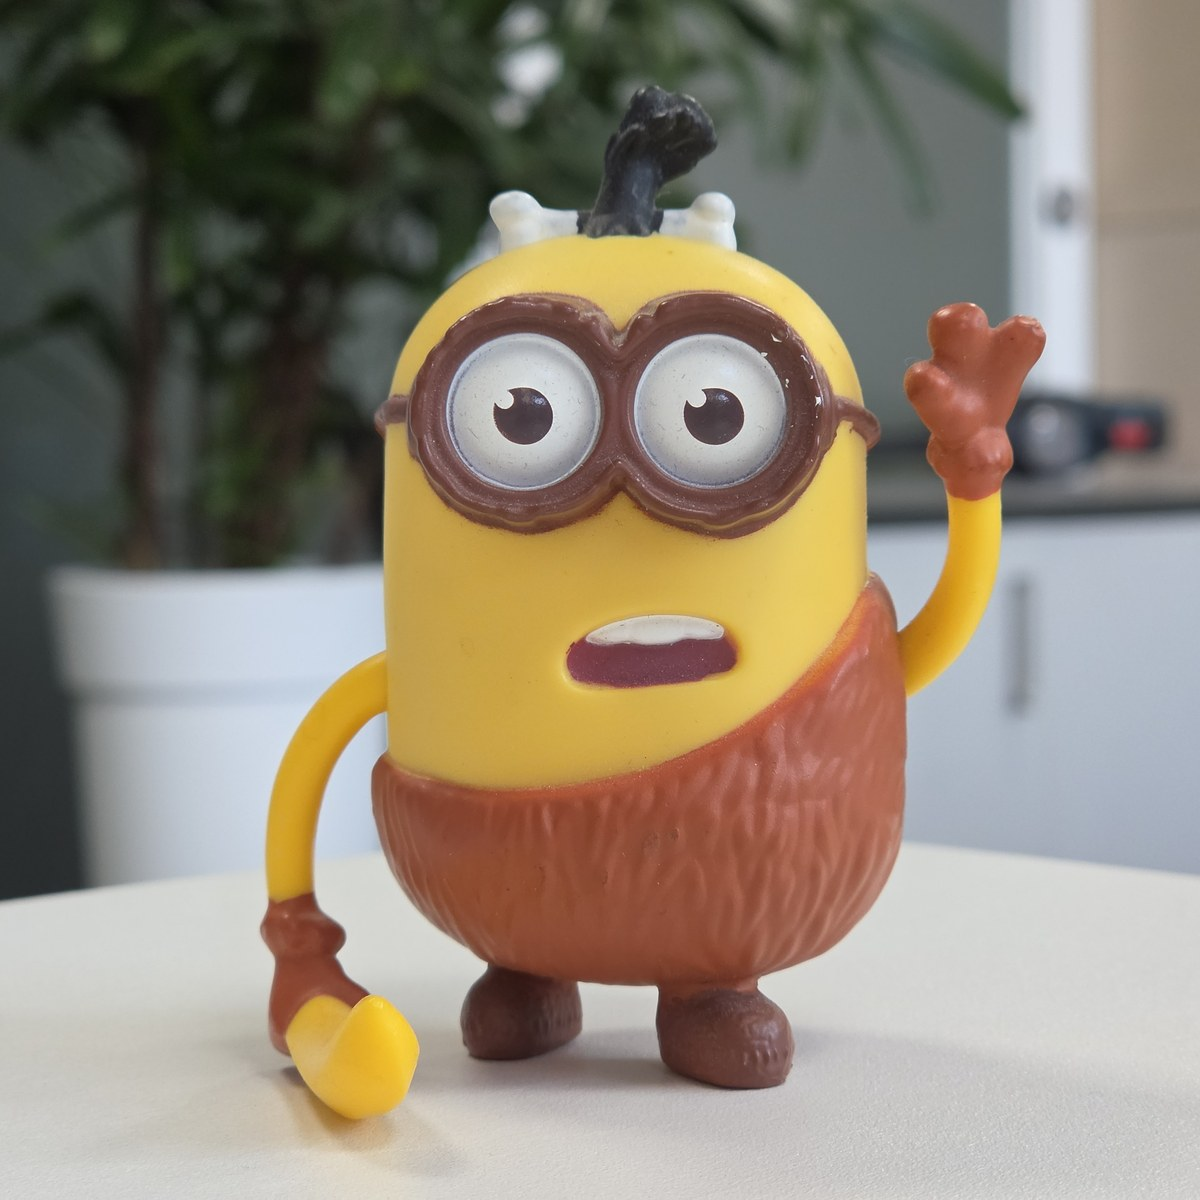
\includegraphics[width=0.485\columnwidth]{figures/fig_draft_final_gap_draft.jpg}};
      \begin{scope}[x={(im.south east)}, y={(im.north west)}]
        \draw[orange, line width=0.8pt] (0.125,0.5792) rectangle (0.5417,0.7458);
      \end{scope}
    \end{tikzpicture} &
    \begin{tikzpicture}
      \node[inner sep=0, anchor=south west] (im) at (0,0)
        {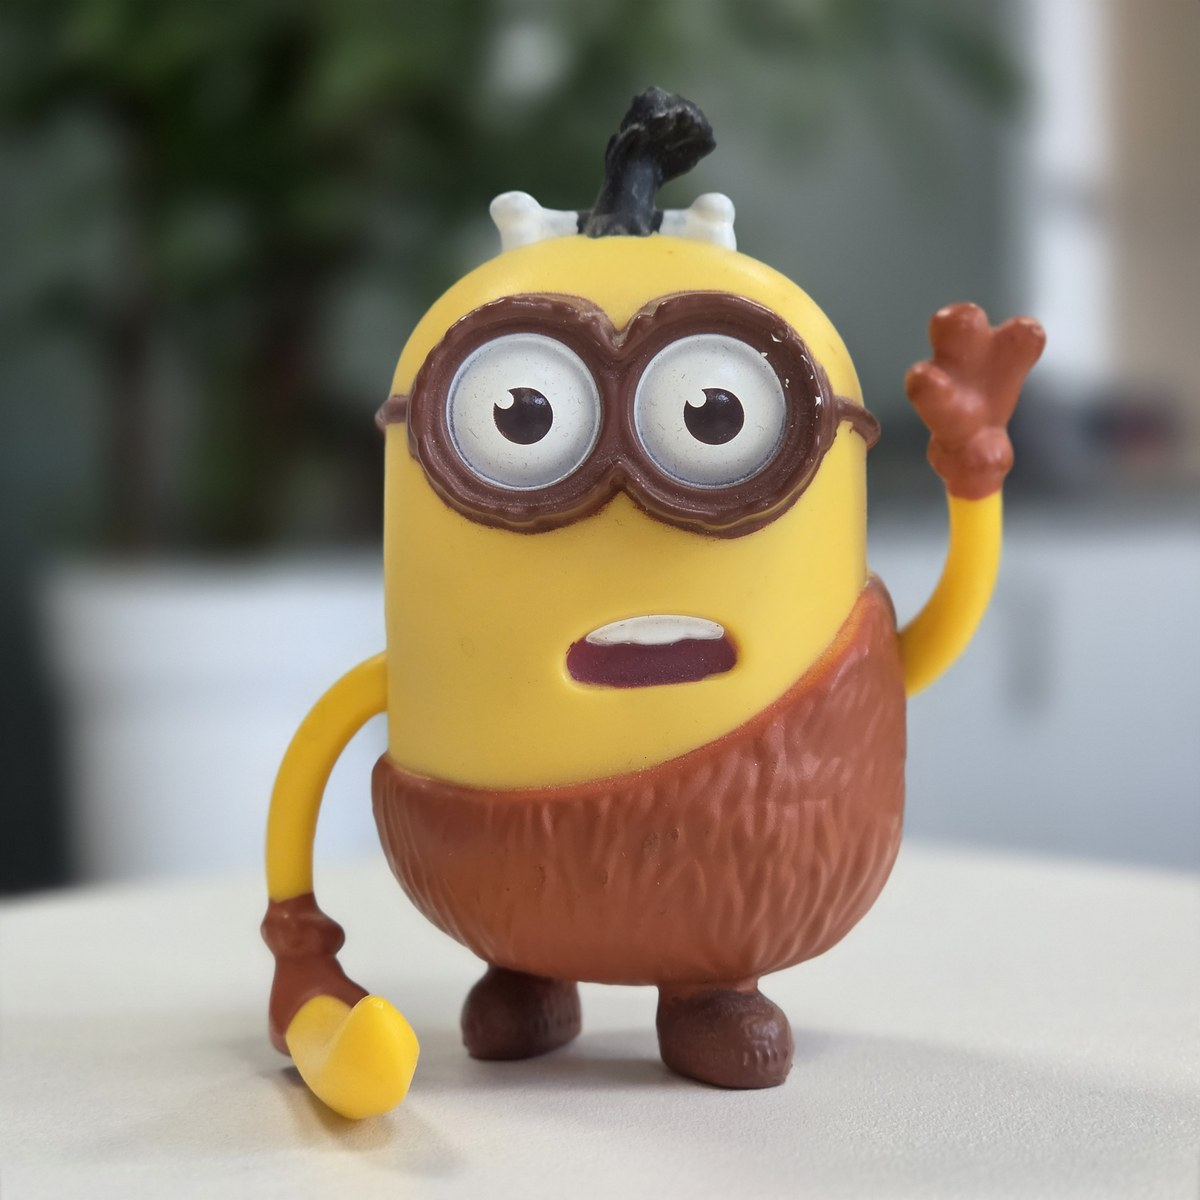
\includegraphics[width=0.485\columnwidth]{figures/fig_draft_final_gap_final.jpg}};
      \begin{scope}[x={(im.south east)}, y={(im.north west)}]
        \draw[orange, line width=0.8pt] (0.125,0.5792) rectangle (0.5417,0.7458);
      \end{scope}
    \end{tikzpicture} \tabularnewline
    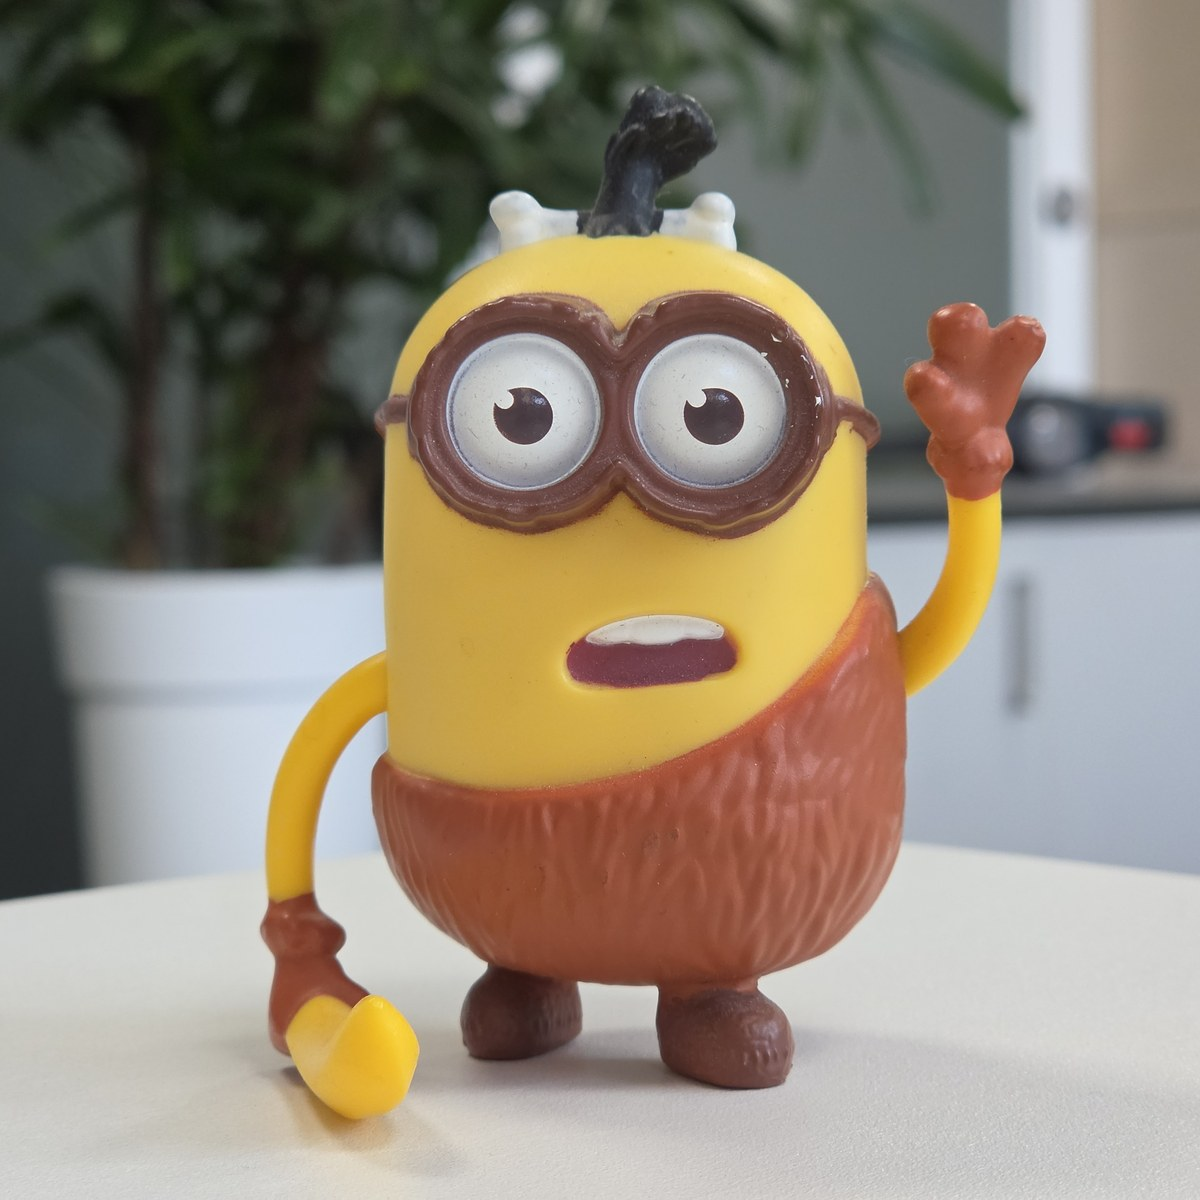
\includegraphics[width=0.485\columnwidth, trim=150 695 550 305, clip]{figures/fig_draft_final_gap_draft.jpg} &
    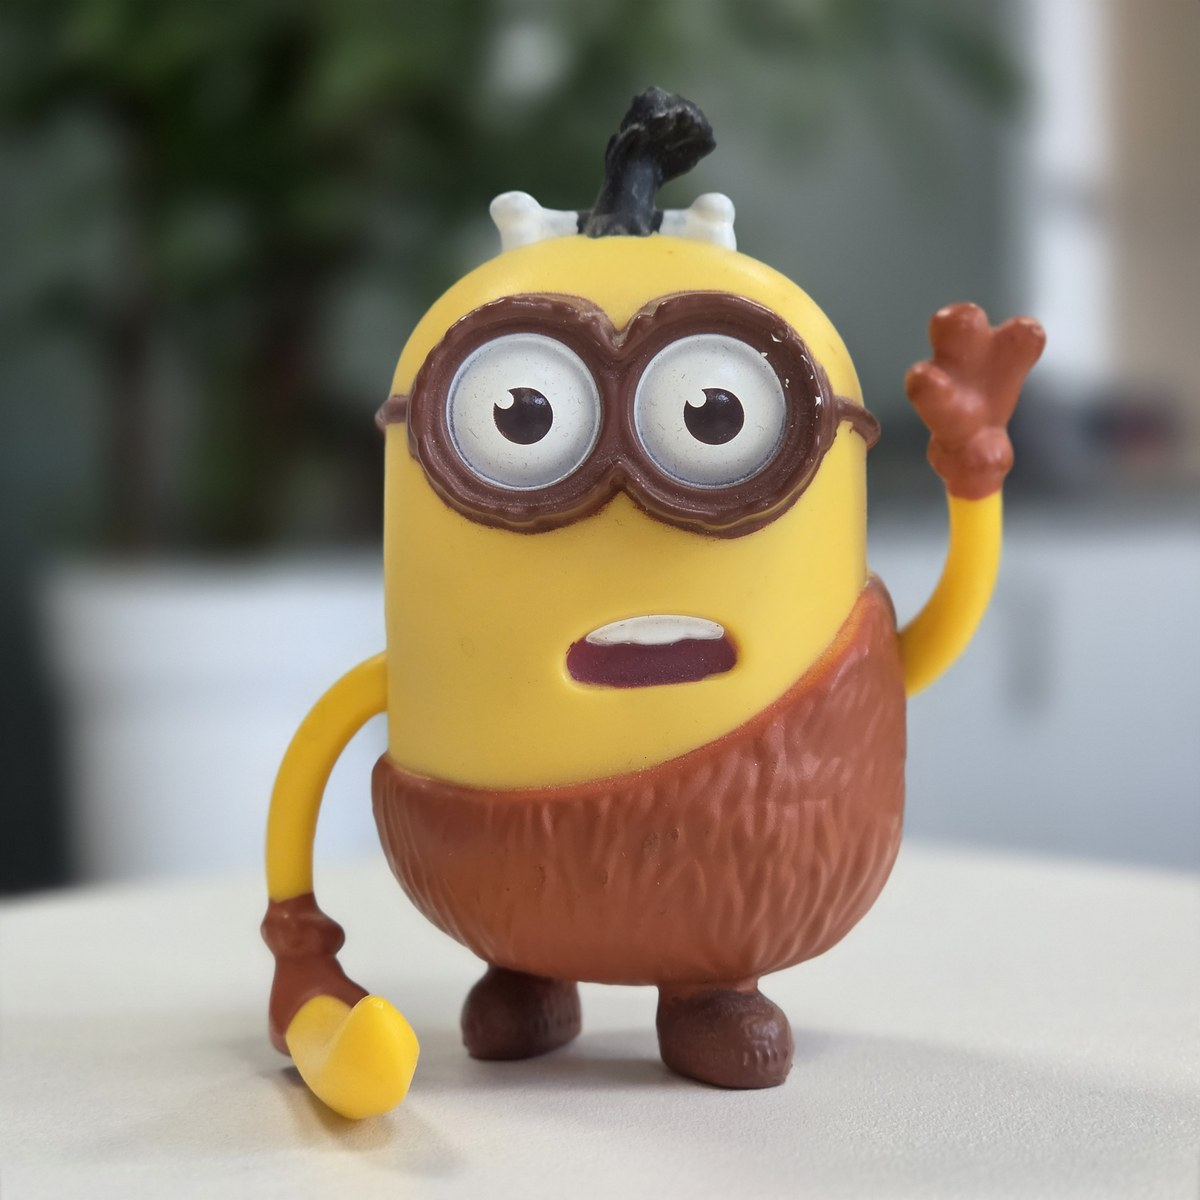
\includegraphics[width=0.485\columnwidth, trim=150 695 550 305, clip]{figures/fig_draft_final_gap_final.jpg} \tabularnewline
    \small Draft image & \small Final image
  \end{tabular}
  \caption{Draft and final images in Portrait mode.}
  \label{fig:draft-final-gap}
\end{figure}
